%----------------------------------------------------------------------------------------
%	PACKAGES AND THEMES
%----------------------------------------------------------------------------------------
\documentclass[aspectratio=169,xcolor=dvipsnames]{beamer}
\usetheme{SimplePlusAIC}

\usepackage{hyperref}
\usepackage{csquotes}
\newcommand{\code}[1]{\texttt{#1}}
\usepackage{graphicx} % Allows including images
\usepackage{booktabs} % Allows the use of \toprule, \midrule and  \bottomrule in tables
\usepackage{svg} %allows using svg figures
\usepackage{tikz}
\usepackage{makecell}
\newcommand*{\defeq}{\stackrel{\text{def}}{=}}
\setbeamertemplate{caption}{\raggedright\insertcaption\par}

%Select the Epilogue font (requires luaLatex or XeLaTex compilers)
\usepackage{fontspec}
\setsansfont{Epilogue}[
    Path=./epilogueFont/,
    Scale=0.9,
    Extension = .ttf,
    UprightFont=*-Regular,
    BoldFont=*-Bold,
    ItalicFont=*-Italic,
    BoldItalicFont=*-BoldItalic
    ]

%----------------------------------------------------------------------------------------
%	TITLE PAGE
%----------------------------------------------------------------------------------------

\title[Char. Musical Sounds with TDA]{Characterizing Musical Sounds with Topological Data Analysis} % The short title appears at the bottom of every slide, the full title is only on the title page
\subtitle{Author: Guo-Wei Wei}

\author[Ivan L. Ihwani]{Presented by: Ivan L. Ihwani}
\institute[SIAM NEWS MARCH 2023]{Department of Mathematics \newline National Central University}
% Your institution as it will appear on the bottom of every slide, maybe shorthand to save space


\date{March 2, 2023} % Date, can be changed to a custom date
%----------------------------------------------------------------------------------------
%	PRESENTATION SLIDES
%----------------------------------------------------------------------------------------

\begin{document}

\begin{frame}[plain]
    % Print the title page as the first slide
    \titlepage
\end{frame}

\begin{frame}{Overview}
    % Throughout your presentation, if you choose to use \section{} and \subsection{} commands, these will automatically be printed on this slide as an overview of your presentation
    \tableofcontents
\end{frame}

%------------------------------------------------
\section{About the Author}
%------------------------------------------------
\begin{frame}{About the Author}
\href{https://users.math.msu.edu/users/weig/}{\textcolor{red}{Guo-Wei Wei}} is a Professor at Michigan State University. His research explores the mathematical foundations of biological science and data science
\end{frame}


%------------------------------------------------
\section{Introduction}
%------------------------------------------------
\begin{frame}{Introduction}
\begin{small}
"Can one hear the shape of a drum?" (Mark Kac, 1966) [4].\\
\vspace{1.5em}
If you hear the sound of a drum, i.e., the set of overtones that it produces, can your infer its shape?\\
\vspace{1.5em}
Mathematically, the essence of this spectral geometry question wonders whether one can uniquely determine a shape based on the eigenvalues of the Laplacian operator that is defined on the shape.
\end{small}
\end{frame}


%-----------------------------------------------
\begin{frame}{Introduction}
\begin{small}
    Many examples of isospectral manifolds are not isometric in settings with two or more dimensions [3]. But the problem is not yet closed, as listeners can indeed discern the shapes of certain geometric types according to their sounds.\\
\vspace{1.5em}
Kac's thought-provoking query also impacts many fields beyond mathematics, including architectural acoustics, audio forensics, pattern recognition, radiology, imaging science, and musical science.
\end{small}
\end{frame}

%------------------------------------------------
\section{Discussion}
%------------------------------------------------

\begin{frame}{Discussion: Modern Musical Instruments}
    Composers commonly use drum sets with multiple pieces of varying sizes (rather than a single drum) to facilitate a tonic harmonic progression: the foundation of harmony in modern music. 
    \begin{figure}[!ht]
\label{drum}
 \centering
 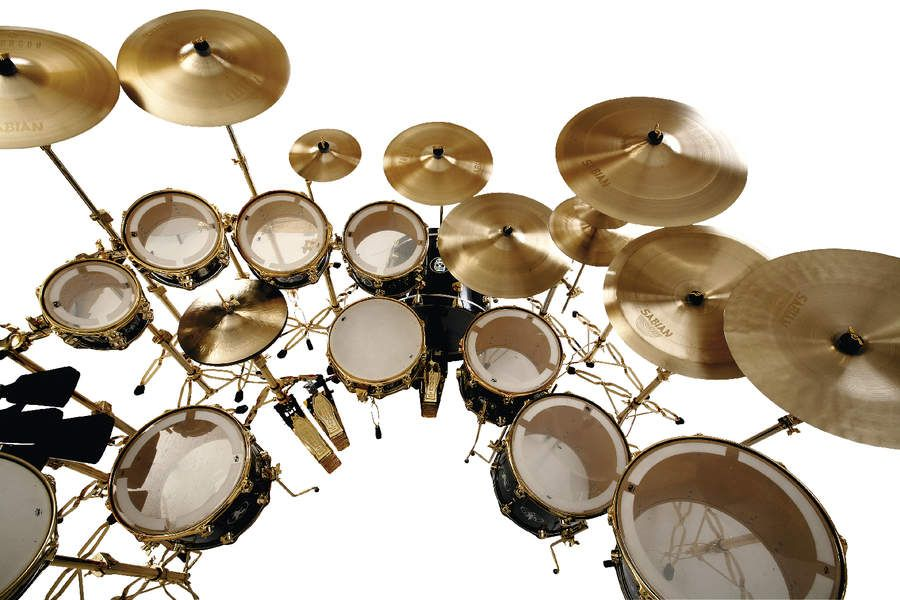
\includegraphics[width=150pt]{images/drum.jpeg}
 \end{figure}
\end{frame}

%--------------------------------------------------------------------------

\begin{frame}{Discussion: Modern Musical Instruments}
    Drum sets can train the human brain to distinguish the overtones of individual drums via a comparative training/learning process that teaches listeners to hear the shape of a particular drum from the set.
    \begin{figure}[!ht]
\label{brain}
 \centering
 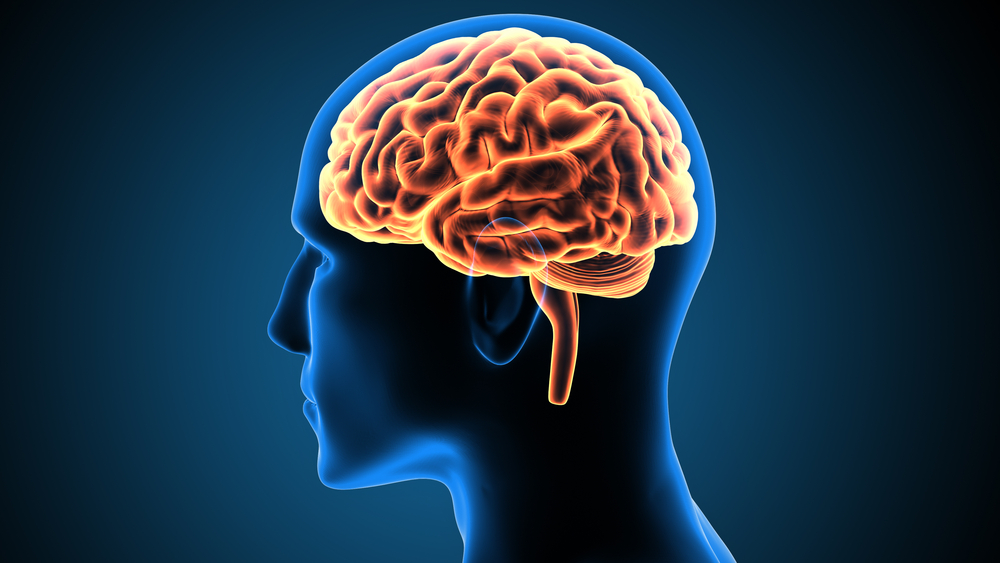
\includegraphics[width=150pt]{images/brain.jpeg}
 \end{figure}
\end{frame}


%----------------------------------------------------------------------

\begin{frame}{Discussion: Progression in \\Musical Instruments}
    \begin{scriptsize}
        To create tonal harmony, artisans in ancient China built a set of 65 chime bells, known as the Zenghouyi Bells, that date back to between 475 and 433 B.C.E., in the Warring States Period (see Figure 1 (a)).
    \end{scriptsize}
    \begin{figure}[!ht]
\label{musical instrument}
 \centering
 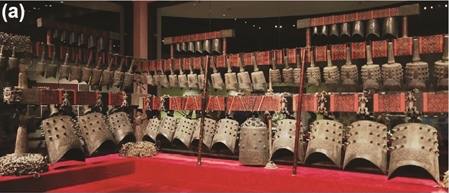
\includegraphics[width=200pt]{images/figure_a.jpeg}
 \caption{Figure 1 (a): The Bianzhong of Marquis Yi of Zeng (Zenghouyi Bells): ancient chime bells that hang on several sets of wooden racks.}
 \end{figure}
\end{frame}

%---------------------------------------------------------------------------------
\begin{frame}{Discussion: Progression in \\Musical Instruments}
\begin{small}
    They designed the shape of each chime bell to produce a distinct sound. The 65 bells gradually vary in size and weight, ranging from 153.4 cm (60.4 inches) to 20.4 cm (8 inches) in height and from 203.6 kg (448.9 pounds) to 2.4 kg (5.3 pounds) in weight. The Zenghouyi Bells comprise a tonal range from C2 to D7 and can play all 12 semitones in the middle of the range, thus enabling different melodies, intervals, and temperaments. 
\end{small}
\end{frame}

%-------------------------------------------------------------------------------------------
\begin{frame}{Discussion: Progression in \\Musical Instruments}
\begin{scriptsize}
    The same design principle appears in many other musical instruments, such as xylophones (Figure 1 (b)), pan flutes (Figure 1 (c)), and pianos (Figure 1 (d)).
\end{scriptsize}
\begin{figure}[!ht]
\label{musical_instrument}
 \centering
 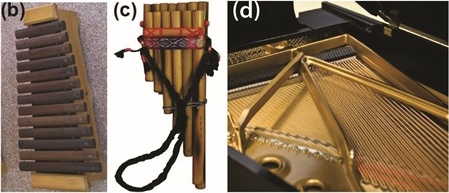
\includegraphics[width=200pt]{images/bcd.jpeg}
 \caption{Figure 1 (b): A xylophone, Figure 1 (c): A pan flute from South America, Figure 1 (d): The strings of a grand piano.}
 \end{figure}
\end{frame}

%------------------------------------------------------------
\begin{frame}{Connection Between Music Instruments \\and Mathematical Filtration}
\begin{small}
    There is a connection between the progression patterns of musical instruments and mathematical filtration, popular technique in modern algebra and topological data analysis (TDA).\\
    \vspace{1.5em}
    TDA is a recent branch of applied mathematics that utilizes topological and geometric concepts to understand and extract topological patterns and structures in data.
\end{small}
\end{frame}

%------------------------------------------------

\begin{frame}{Persistent Homology}
\begin{small}
The main workshare of TDA is persistent homology [2, 6], an extension of algebraic topology that employs filtration to create a mathematical microscopy of a point cloud. Persistent homology delineates the shape of data through comparative analysis of the topological invariant changes that are induced by filtration [6]. \\
\vspace{1.5em}
Persistent homology has become one of the most powerful tools for simplifying the geometric complexity and reducing the high dimensionality of biomolecular interactions [5], ultimately \textcolor{red}{revolutionizing drug discovery} and \textcolor{red}{effectively forecasting emerging viral variants}.
\end{small}
\end{frame}

%-----------------------------------------------------------------------------------------
\begin{frame}{Result of Persistent Homology}
\begin{small}
    However, persistent homology is not directly applicable to the tonal analysis of chime bells. First, one may regard the collection of chime bells as the result of a set of evolving chime bell manifolds, rather than the result of point cloud filtration. Additionally, no change in topological invariants is associated with the homotopic shape evolution of chime bells. And finally, persistent homology cannot present a frequency or tonal analysis of chime bells or many other musical instruments.
\end{small}
\end{frame}
%-------------------------------------------------------------------------------------------
\begin{frame}{Point Cloud}
    \begin{small}
        In computer science and computational geometry, a point cloud is a collection of data points in three-dimensional space that represent the coordinates and attributes (such as color or intensity) of objects or surfaces captured by a sensor, such as a lidar scanner, a depth camera, or a photogrammetric system.
    \end{small}
    \begin{figure}[!ht]
\label{pointcloud}
 \centering
 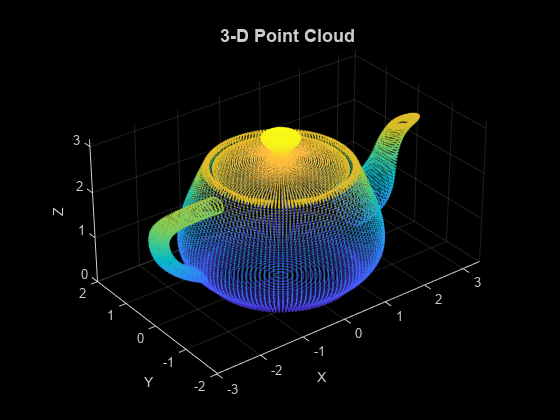
\includegraphics[width=120pt]{images/pointcloud.png}
 \caption{Point Cloud Example}
 \end{figure}
\end{frame}

%-------------------------------------------------------------------------------------------
\section{The Proposed Method}
%----------------------------------------------------------------------------------------
\begin{frame}{The Proposed Method}
\begin{small}
    Researchers proposed an evolutionary de Rham-Hodge method [1] as a multiscale generalization of classical de Rham-Hodge theory to provide a multiscale geometric and topological analysis of filtration-induced manifolds, which enables the characterization of tonal evolution of chime bells by defining a family of evolutionary Hodge Laplacians with the help of these manifolds, revealing the full set of topological invariants in their kernel or null space dimensions.
\end{small}
\end{frame}
%------------------------------------------------

\begin{frame}{Illustration of Filtration and \\Persistent Laplacian Spectra}
\begin{figure}[!ht]
\label{filtration}
 \centering
 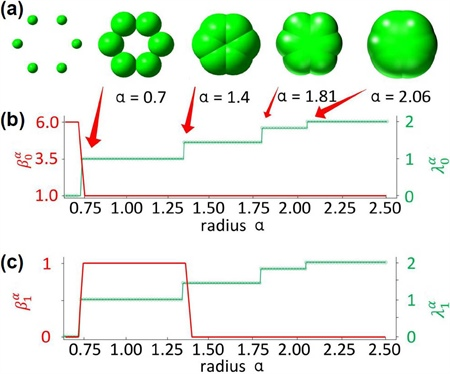
\includegraphics[width=120pt]{images/filtration.jpeg}
 \caption{Figure (2a) Filtration of a point cloud. (2b-2c) Persistent Laplacian analysis of the point cloud. Here, $\beta^{\alpha}_{j}$ and $\lambda^{\alpha}_{j}$ ($j=0,1$) are respectively persistent Betti-$j$ numbers and the first nonzero eigenvalues of the $j$th persistent Laplacian. $\lambda^{\alpha}_{j}$ captures the homotopic shape evolution of data (see the frequency changes after $\alpha=1.5$), which is not reflected in $\beta^{\alpha}_{j}$.}
 \end{figure}
\end{frame}


%------------------------------------------------
\begin{frame}{The Proposed Method}
\begin{small}
    The point cloud counterpart of the evolutionary de Rham-Hodge method on manifolds is called persistent spectral graph (also known as persistent Laplacians) on simplicial complexes [7, 8]. Like the evolutionary de Rham-Hodge method, persistent Laplacians both return the full set of topological invariants in their harmonic spectra (as does persistent homology) and capture the homotopic shape evolution of data during filtration in their first non-harmonic spectra (see Figures 2b and 2c); persistent homology cannot handle this latter task.
    \end{small}
\end{frame}

%-------------------------------------------------------------------------------------
\section{Summary}
%--------------------------------------------------------------------------------------
\begin{frame}{Summary}
    Sheaf theory created a generalization of persistent Laplacians, and the resulting persistent sheaf Laplacians enable the embedding of heterogeneous characters in topological invariants (e.g., encoding non-geometric information in a geometry-based simplicial complex) [10]. Persistent path Laplacian, another generalization that is built from the path complex, are designed for directed graphs and directed networks [9]. These new persistent topological Laplacians lay a mathematical foundation for tonal analysis in musical science and significantly extend the applicable domain and power of TDA.
\end{frame}


%-----------------------------------------------------------
%\begin{frame}{Cox Rings of Linear Quotients}
 %   \begin{itemize}
  %      \item This \textcolor{blue}{\href{https://github.com/micjoswig/oscar-notebooks/blob/master/SIAM-News/Cox_rings_of_linear_quotients.ipynb}{example}} is related to the Cox ring of the \textcolor{blue}{Linear Quotient}. 
   %     \item Here, we must compute a certain \textcolor{blue}{invariant ring} and endow it with a nonstandard grading by a theorem of Ivan Arzhantsev and Sergey Gaĭfullin (mathematician in the Invariant Theory field). 
    %    \item Calculating this ring aids in examining the birational geometry of a linear quotient.
     %   \item \textbf{OSCAR} offers all the essential tools for efficiently handling matrix groups and their invariant theory.
    %\end{itemize}
%\end{frame}
%-------------------------------------------------------
%\begin{frame}{Table}
 %   \begin{table}
  %      \begin{tabular}{l l l}
   %         \toprule
    %        \textbf{Treatments} & \textbf{Response 1} & \textbf{Response 2} \\
     %       \midrule
      %      Treatment 1         & 0.0003262           & 0.562               \\
     %       Treatment 2         & 0.0015681           & 0.910               \\
     %       Treatment 3         & 0.0009271           & 0.296               \\
     %       \bottomrule
    %    \end{tabular}
    %    \caption{Table caption}
   % \end{table}
%\end{frame}

%------------------------------------------------

%\begin{frame}{Theorem}
 %   \begin{theorem}[Mass--energy equivalence]
 %       $E = mc^2$
 %   \end{theorem}
 %   \begin{equation}
 %       c^{2} = a^{2} + b^{2}
 %   \end{equation}
%\end{frame}

%------------------------------------------------

%\begin{frame}{Figure}
    %Uncomment the code on this slide to include your own image %from the same directory as the template .TeX file.
    %\begin{figure}
    %\includegraphics[width=0.8\linewidth]{test}
    %\end{figure}
%\end{frame}

%------------------------------------------------

%\begin{frame}[fragile] % Need to use the fragile option when verbatim is used in the slide
%    \frametitle{Citation}
 %   An example of the \verb|\cite| command to cite within the presentation:\\~

  %  This statement requires citation \cite{p1}.
%\end{frame}

%------------------------------------------------

\begin{frame}{References}
    % Beamer does not support BibTeX so references must be inserted manually as below
    \footnotesize{
        \begin{thebibliography}{99}
            \bibitem[Chen, J., Zhao, R., Tong, Y., Wei, G.-W., 2021]{p1} Chen, J., Zhao, R., Tong, Y., \& Wei, G.-W. (2021)
            \newblock Evolutionary de Rham-Hodge method
            \newblock \emph{Discrete Contin. Dyn. Syst. Ser. B,}  26 (7), 3785-3821.
        \end{thebibliography}
        \begin{thebibliography}{99}
            \bibitem[Edelsbrunner, H., \& Harer, J., 2008]{p1} Edelsbrunner, H., \& Harer, J. (2008)
            \newblock Persistent homology — a survey
            \newblock \emph{Contemp. Math.,} 453, 257-282.
        \end{thebibliography}
        \begin{thebibliography}{99}
            \bibitem[Gordon, C., Webb, D., \& Wolpert, S., 1992]{p1} Gordon, C., Webb, D., \& Wolpert, S. (1992)
            \newblock Isospectral plane domains and surfaces via Riemannian orbifolds
            \newblock \emph{Inventiones Math.,} 110(1), 1-22.
        \end{thebibliography}
        \begin{thebibliography}{99}
            \bibitem[Kac, M., 1966]{p1} Kac, M. (1966)
            \newblock Can one hear the shape of a drum?
            \newblock \emph{Am. Math. Mon.,} 73(4P2), 1-23.
        \end{thebibliography}
    }
\end{frame}

\begin{frame}{References}
    % Beamer does not support BibTeX so references must be inserted manually as below
    \footnotesize{
        \begin{thebibliography}{99}
            \bibitem[Liu, J., Xia, K.-L., Wu, J., Yau, S.S.-T., \& Wei, G.-W., 2022]{p1} Liu, J., Xia, K.-L., Wu, J., Yau, S.S.-T., \& Wei, G.-W. (2022)
            \newblock Biomolecular topology: Modelling and analysis
            \newblock \emph{Acta Math. Sin. Engl.,} 38(10), 1901-1938.
        \end{thebibliography}
        \begin{thebibliography}{99}
            \bibitem[Lum, P.Y., Singh, G., Lehman, A., Ishkanov, T., Vejdemo-Johansson, M., Alagappan, M., \& Carlsson, G., 2013]{p1} Lum, P.Y., Singh, G., Lehman, A., Ishkanov, T., Vejdemo-Johansson, M., Alagappan, M., \& Carlsson, G. (2013)
            \newblock Extracting insights from the shape of complex data using topology
            \newblock \emph{ Sci. Rep.,} 3(1), 1-8.
        \end{thebibliography}
        \begin{thebibliography}{99}
            \bibitem[Mémoli, F., Wan, Z., \& Wang, Y., 2022]{p1} Mémoli, F., Wan, Z., \& Wang, Y. (2022)
            \newblock Persistent Laplacians: Properties, algorithms and implications
            \newblock \emph{SIAM J. Math. Data Sci.,} 4(2), 858-884.
        \end{thebibliography}
        \begin{thebibliography}{99}
            \bibitem[Wang, R., Nguyen, D.D., \& Wei, G.-W., 2020]{p1} Wang, R., Nguyen, D.D., \& Wei, G.-W. (2020)
            \newblock Persistent spectral graph
            \newblock \emph{Int. J. Numer. Methods in Biomed. Eng.,} 36(9), e3376.
        \end{thebibliography}
    }
\end{frame}

\begin{frame}{References}
    % Beamer does not support BibTeX so references must be inserted manually as below
    \footnotesize{
        \begin{thebibliography}{99}
            \bibitem[Wang, R., \& Wei, G.-W., 2023]{p1}   Wang, R., \& Wei, G.-W. (2023)
            \newblock Persistent path Laplacians
            \newblock \emph{Found. Data Sci.,}5, 26-55.
        \end{thebibliography}
        \begin{thebibliography}{99}
            \bibitem[Wei, X., \& Wei, G.-W., 2021]{p1} Wei, X., \& Wei, G.-W. (2021)
            \newblock Persistent sheaf Laplacians
            \newblock \emph{Preprint,} arXiv:2112.10906.
        \end{thebibliography}
}
\end{frame}

%------------------------------------------------

\begin{frame}
    \Huge{\centerline{\textbf{Thank You}}}
\end{frame}

%----------------------------------------------------------------------------------------
\end{document}